\documentclass[a4paper,twoside,12pt]{article}
\usepackage{zed-cm}
\usepackage{graphicx}
\graphicspath{ {./images/} }
\usepackage[export]{adjustbox}
\usepackage[nottoc,numbib]{tocbibind}
%\usepackage{hyperref}
\markboth{Draft}{Version 0.1}
\pagestyle{myheadings}
\begin{document}
\parskip 10 pt
\parindent 0 pt

\def\Slash{\slash\hspace{0pt}}

\title{OCI Image Format}

\author{Glyn Normington}

\maketitle
% The following three commands ensure the title page is without a page number but page numbering starts here.
% Page numbers appear on subsequent pages, and are roman until the main body, which starts again at arabic 1.
\thispagestyle{empty}
\pagenumbering{roman}
\setcounter{page}{1}

%=============================================================================

This document provides a formal model of some aspects of the \textit{OCI image format}. It describes the objects which make
up an OCI repository and how content addressing is used to refer to these objects.

%I am indebted to Chris Frost and Steve Powell for their helpful feedback.

% Alt-Cmd-M -- \emph{}
% Alt-Cmd-Z -- \zed{}
% Alt-Cmd-X -- \axdef{}
% Alt-Cmd-S -- \schema{}
% Alt-Shift-Cmd-T -- \texttt{}

% Type checking hacks
\newcommand{\true}{true}
\newcommand{\false}{false}
\renewcommand{\emptyset}{\varnothing}
%=============================================================================

\clearpage
\tableofcontents

\cleardoublepage
\pagenumbering{arabic}
\setcounter{page}{1}

%=============================================================================
\section{Introduction}

Docker Inc.\ (\cite{docker}) introduced \textit{container images} and \textit{registries} to hold them and these were later standardised as part of the Open Container Initiative (\cite{oci}). The reader is assumed to have a basic understanding of how images are used.

Registries are named collections of \textit{repositories}. The relationship is described formally in \textit{Image Registries} (\cite{registries}).

This document models how image are represented and stored in repositories. This is based on the \textit{OCI Image Format Specification} (\cite{ociimage}). It does not cover all details, but aims to provide an overview of how images are structured as layers and gathered into a repository. The following diagram shows the main objects that are modelled.

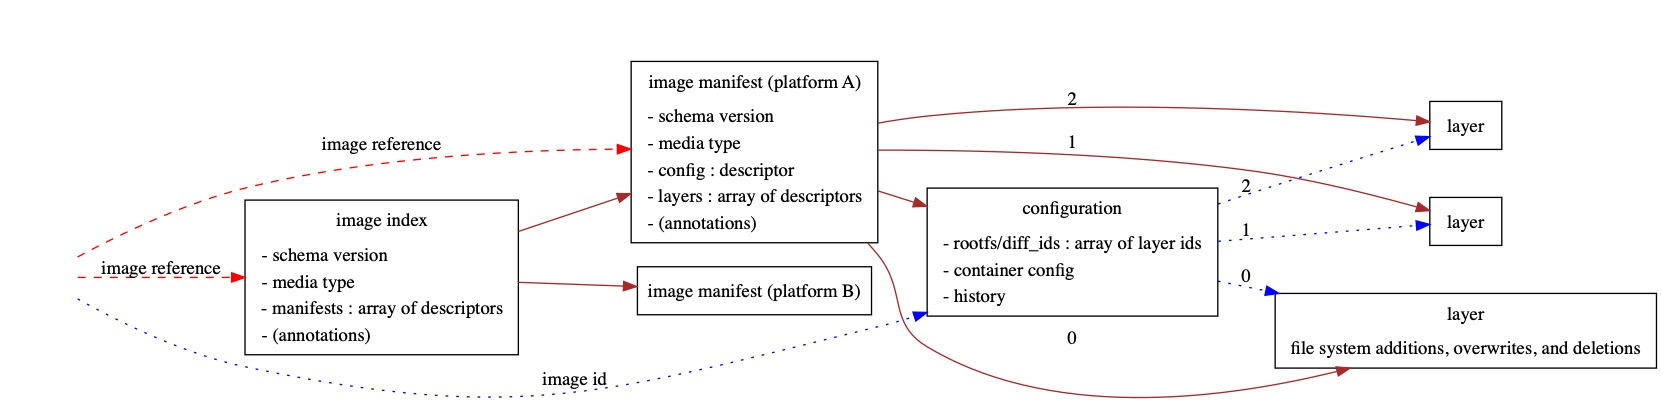
\includegraphics[width=17cm,left]{ociimage.jpeg}

The Z specification language is used to describe the model, but sufficient English text is also provided that readers who do not know Z should be able to get a reasonable idea of what's going on. The appendix contains a summary of the Z notation.
For more information about Z, please consult the Z Manual (\cite{zman}).
The model was type checked using \texttt{fuzz} (\cite{fuzz}).

%=============================================================================
\newpage
\section{Content Addressing}

Before we describe the objects which make up a repository, we model how objects refers to each other using \textit{content addressing}.
In content addressing, a collision resistant function\footnote{collision resistant functions are designed so that it is extremely unlikely that distinct inputs produce the same output} is applied to the content of an object to produce a content address which can be used to refer to the object.

OCI uses a form of \textit{content address}, known as a \textit{digest}, which is a cryptographic hash of the \textit{compressed} content of an object.
\begin{zed}
[ Digest ] 
\end{zed}

OCI also uses another form of content address, known as an \textit{id}, which is a cryptographic hash of the \textit{uncompressed} content of an object.
\begin{zed}
[ Id ] 
\end{zed}

Content addressable storage (CAS) in a repository has a collection of objects uniquely identified by digest and, sometimes, by id. Each object has a ``raw'' (possibly compressed) size in bytes.
\begin{schema}{CAS}[Object]
  deref : Digest \pinj Object \\
  identify : Id \pinj Object \\
  size : Digest \pfun \nat \\
\where
  \ran identify \subseteq \ran deref \\
  \dom deref = \dom size \\
\end{schema}

As well as addressing objects by digest, some intra-repository references use \textit{descriptors}. A descriptor augments a digest with extra descriptive information: media type, URLs, and strings (used in annotations), which are not modelled further.
\begin{zed}
[ MediaType, URL, String ] 
\end{zed}
A media type is used to distinguish between certain types of objects in a repository. URLs indicate where certain objects are hosted in a network. Annotations provide arbitrary metadata for certain objects.

A descriptor is a way of referring to an object in the same repository using a digest, a media type, a ``raw'' size, and zero or more URLs and annotations.
\begin{schema}{Descriptor}
  digest : Digest \\
  mediaType : MediaType \\
  size : \nat \\
  urls : \seq URL \\
  annotations : String \pfun String \\
\end{schema}

We will model a repository as a collection of content addressable objects, which we will introduce in turn, along with their media types.
These objects are change sets, image configurations, image manifests, and image indices.

%=============================================================================
\newpage
\section{Change Sets (``Layers'')}

A changeset, or ``layer'', is a means of creating a root file system for a container based on an image.

File system paths and files (including directories) are modelled in terms of their usage, but not their implementation.
\begin{zed}
[ FSPath, File ] 
\end{zed}

We introduce a simple model of a file system which will be sufficient to show how the file system of an image is built from layers.

A simplified file system is a collection of files indexed by file system path.
\begin{schema}{FS}
  fs : FSPath \pfun File \\
\end{schema}
No mention is made of the hierarchical nature of file system paths. File modes and attributes and symbolic and hard links are not modelled.

An empty file system has no files.
\begin{zed}
  EmptyFS \defs [ FS | fs = \emptyset ]
\end{zed}

An \textit{image layer file system changeset}, informally known as a ``layer'', describes a particular type of modification to a file system where some files are first of all removed and then files are added or replaced.
\begin{schema}{ChangeSet}
  remove : \power FSPath \\
  add : FSPath \pfun File \\
\end{schema}

There is a media type for changesets which will be used in descriptors that reference changesets.
\begin{axdef}
  LAYER : MediaType \\
\end{axdef}

A changeset is applied to a file system by removing files according to the changeset and then adding (or replacing) file according to the changeset.
\begin{schema}{ChangeSetApply}
  \Delta FS \\
  c? : ChangeSet \\
\where
   fs' = (c?.remove \ndres fs) \oplus c?.add \\ 
\end{schema}

Applying a changeset to an empty file system results in a file system containing of just the additions from the changeset. So a sequence of changesets can be applied in turn starting with an empty file system to produce the ``root'' file system for a particular \textit{container}.

The remainder of this document does not concern itself with combining changesets, except that it will show how an image refers to a sequence of 
changesets which can, as we have just seen, be used to form the root file system for each container constructed from the image.

\subsection{Image Repositories (part 1 of 4)}

We can now start to describe image repositories in terms of change sets. Other objects in an image repository will be described later.

An image repository has a content addressable collection of change sets.
\begin{schema}{RepositoryChangeSets}
  changesets: CAS[ChangeSet] \\
\end{schema}
This will make more sense once we start to add other objects to the repository.

%=============================================================================
\newpage
\section{Image Configurations}

Container configurations and (image history) logs are used by container configurations, but are not modelled further.
\begin{zed}
[ ContainerCfg, Log ] 
\end{zed}

There is a media type for image configurations which will be used in descriptors that reference image configurations.
\begin{axdef}
  CONFIG : MediaType \\
\end{axdef}

An image configuration refers to the changesets (or ``layers'', of which there must be at least one) of an image and records the container configuration and history of the image.
\begin{schema}{Config}
  changesets : \seq_1 Id \\
  ccfg: ContainerCfg \\
  history: \seq Log \\
\end{schema}

\subsection{Image Repositories (part 2 of 4)}

We now add configurations to our description of an image repository and see how configurations relate to change sets. Other objects in an image repository will be described later.

An image repository has a content addressable collection of change sets and configurations addressed by id.
\begin{schema}{RepositoryConfigsAndLayers}
  RepositoryChangeSets \\
  configs: CAS[Config] \\
  ids : \power Id \\
  digests : \power Digest \\
\where
  \forall cfg : \ran configs.deref @ \ran cfg.changesets \subseteq \dom changesets.identify \\
  \langle \dom changesets.identify, \dom configs.identify \rangle \partition ids \\
  \exists other : \power Digest @ \\
  \t1 \langle \dom changesets.deref, \dom configs.deref, other \rangle \partition digests \\
\end{schema}
All configurations refer to valid changeset ids.

Ids and digests are partitioned between configurations and changesets (and, in the case of digests, other objects still to be introduced).
That is, each id and each digest refers to at most one object in content addressable storage.

The next step is to introduce the central object in a repository: the \textit{image manifest}.

%=============================================================================
\newpage
\section{Image Manifests}

The central object in an image repository is the \textit{image manifest} which describes a single image.

Image manifests have schema versions, which are not modelled further.
\begin{zed}
[ SchemaVersion ] 
\end{zed}

There is a media type for image manifests which is used both in image manifests and in descriptors that reference them.
\begin{axdef}
  IMAGE\_MANIFEST : MediaType \\
\end{axdef}

An image manifest refers to an image configuration and at least one changeset (or ``layer'').
\begin{schema}{Manifest}
  schemaVersion : SchemaVersion \\
  mediaType : MediaType \\
  config : Descriptor \\
  changesets : \seq_1 Descriptor \\
  annotations : String \pfun String \\
\where
  mediaType = IMAGE\_MANIFEST \\
\end{schema}

\subsection{Image Repositories (part 3 of 4)}

We extend our model of an image repository to include image manifests.
\begin{schema}{RepositoryManifestsConfigsAndLayers}
  RepositoryConfigsAndLayers \\
  manifests: CAS[Manifest] \\
\where
  manifests.identify = \emptyset \\
\also
  \exists other : \power Digest @ \\
  \t1 \langle \dom changesets.deref, \dom configs.deref, \\
  \t2 \dom manifests.deref, other  \rangle \partition digests \\
\also
  \forall man : \ran manifests.deref @ \\
   \t1 man.mediaType = IMAGE\_MANIFEST \land \\
   \t1 man.config.mediaType = CONFIG \land \\
   \t1 man.config.digest \in \dom configs.deref \land \\
   \t1 man.config.size = configs.size~man.config.digest \land \\
   \t1 (\forall cs : \ran man.changesets @ \\
     \t2 cs.mediaType = LAYER \land \\
     \t2 cs.digest \in \dom changesets.deref \land \\
     \t2 cs.size = changesets.size~cs.digest) \\
\end{schema}
Manifests do not have ids.

Also, content addresses in the form of digests are partitioned between changesets, configs, manifests, and other objects (soon to be introduced).
That is, each digest refers to at most one object in content addressable storage.

Also, all manifests have an appropriate media type and valid configuration and layer descriptors.

%=============================================================================
\newpage
\section{Image Indices}

To complete our description of image repositories, we add another object, the \textit{image index}. The main purpose of an image index is to
enable a repository to contain multiple versions of an image for multiple platforms.

Image indices use extended descriptors which include platform information, which is not modelled further.
\begin{zed}
[ Platform ] 
\end{zed}

There is a media type for image indices which is used both in image indices and in descriptors that reference them.
\begin{axdef}
  IMAGE\_INDEX : MediaType \\
\end{axdef}

A manifest descriptor is a descriptor with an additional property denoting a platform.
\begin{schema}{ManifestDescriptor}
  Descriptor \\
  platform : Platform \\
\where
  mediaType \in \{ IMAGE\_MANIFEST, IMAGE\_INDEX \} \\
\end{schema}
A manifest descriptor may refer to image manifests or image indices.

An image index refers to zero or more image manifests and/or image indices.
\begin{schema}{Index}
  schemaVersion : SchemaVersion \\
  mediaType : MediaType \\
  manifests : \seq ManifestDescriptor \\
  annotations : String \pfun String \\
\where
  mediaType = IMAGE\_INDEX \\
\end{schema}

\subsection{Image Repositories (part 4 of 4)}

We can now complete our model of image repositories.

An image repository is a content addressable collection of change sets, configurations, image manifests, and image indices.
\begin{schema}{Repository}
  RepositoryManifestsConfigsAndLayers \\
  indices: CAS[Index] \\
\where
  indices.identify = \emptyset \\
\also
  \langle \dom changesets.deref, \dom configs.deref, \\
  \t1 \dom manifests.deref, \dom indices.deref  \rangle \partition digests \\
\also
  \forall idx : \ran indices.deref @ \\
  \t1 idx.mediaType = IMAGE\_INDEX \land \\
  \t1 (\forall man : \ran idx.manifests @ \\
    \t2 (man.digest \in \dom manifests.deref \land \\
    \t2 man.size = manifests.size~man.digest) \lor \\
    \t2 (man.digest \in \dom indices.deref \land \\
    \t2 man.size = indices.size~man.digest)) \\
\also
  \exists next : Index \rel Index | \forall i, j : Index | i \mapsto j \in next @ \\
  \t1 (\exists m : \ran i.manifests @ indices.deref~m.digest = j) @ \\
  \t2 next\plus \cap \id Index = \emptyset \\
\end{schema}
Image indices do not have ids.

Also, content addresses in the form of digests are partitioned between changesets, configs, manifests, and indices.
That is, each digest refers to at most one object in content addressable storage.

Also, all image indices have an appropriate media type and valid manifest descriptors (referring to image manifests and/or other image indices).

Also, there are no cycles of image indices.

%%%%%%%%%%%%%%%%%%%%%%%%%%%%%%%%%%%%%%%%%%%%%%%
%   A P P E N D I C E S
%%%%%%%%%%%%%%%%%%%%%%%%%%%%%%%%%%%%%%%%%%%%%%%

\clearpage

\appendix

%=============================================================================
%   B I B L I O G R A P H Y
%=============================================================================
\newpage
\begin{flushleft}
\begin{thebibliography}{99}
\label{sec:references}
% `99' is a picture of the generated numeric references -- they are two digits in this bibliography
% If we had a hundred or more we would have used 999, or whatever.

%%  Example bibliography entry:
%\bibitem{knuth76}                                                        % citation callout, e.g.: \cite{knuth76}
%  Donald E. Knuth,                                                        % author
%  \emph{The computer as Master Mind}.                    % title
%  J. Recreational Mathematics, Vol.~9(1), 1976-1977. % publisher, or journal, volume and date

\bibitem{docker}
  Various authors,
  \emph{Docker Inc.},
  \texttt{https://www.docker.com/}.

\bibitem{oci}
  Various authors,
  \emph{Open Container Initiative},
  \texttt{https://www.opencontainers.org/}.

\bibitem{registries}
  Glyn Normington,
  \emph{Image Registries},
  \texttt{https://github.com/glyn/riff-specs/raw/master/distribution/}\\\texttt{distribution.pdf}.

\bibitem{ociimage}
  Various authors,
  \emph{OCI Image Format Specification},
  \texttt{https://github.com/opencontainers/image-spec/blob/master/spec.md}.

\bibitem{zman}
  Mike Spivey,
  \emph{The Z Manual},
  \texttt{https://www.cs.umd.edu/ mvz/handouts/z-manual.pdf}.

\bibitem{fuzz}
  Mike Spivey,
  \emph{The fuzz type-checker for Z},
  \texttt{https://bitbucket.org/Spivey/fuzz}.


\end{thebibliography}
\end{flushleft}

%=============================================================================
%   Z   N O T A T I O N
%=============================================================================
\newpage
\section{Z Notation}
\label{sec:znot}
{\scriptsize
\makeatletter % the following code is taken from Mike Spivey's zed.tex

\def\symtab{\setbox0=\vbox\bgroup \def\\{\cr}
        \halign\bgroup\strut$##$\hfil&\quad##\hfil\cr}
\def\endsymtab{\crcr\egroup\egroup
        \dimen0=\ht0 \divide\dimen0 by2 \advance\dimen0 by\ht\strutbox
        \splittopskip=\ht\strutbox \vbadness=10000
        \predisplaypenalty=0
        $$\halign{##\cr\hbox to\linewidth{%
                \valign{##\vfil\cr
                        \setbox1=\vsplit0 to\dimen0 \unvbox1\cr
                        \noalign{\hfil}\unvbox0\cr
                        \noalign{\hfil}}}\cr
                \noalign{\prevdepth=\dp\strutbox}}$$
        \global\@ignoretrue}

\makeatother

Numbers:
\begin{symtab}
        \nat & \verb/Natural numbers/ \{\verb/0,1,.../\} \\
%       \num & \verb/Integers (...,-1,0,1,...)/ \\
%       \nat_1 & \verb/Positive natural numbers/ \\
%       \upto & \verb/integral range/ \\
%       + & \verb/Addition/\quad\hfill 3 \\
%       - & \verb/Subtraction/\quad\hfill 3 \\
%       * & \verb/Multiply/\quad\hfill 4 \\
%       \div & \verb/Remainder/\quad\hfill 4 \\
%       \mod & \verb/Modulus/\quad\hfill 4 \\
%       < & \verb/Less than/ \\
%       > & \verb/Greater than/ \\
%       \leq & \verb/Less than or equal/ \\
%       \geq & \verb/Greater than or equal/ \\
%       \neq & \verb/Inequality/ \\
\end{symtab}
Propositional logic and the schema calculus:
\begin{symtab}
%       \lnot & \verb/Not/ \\
        \ldots\land\ldots & \verb/And/ \\
        \ldots\lor\ldots & \verb/Or/ \\
        \ldots\implies\ldots & \verb/Implies/ \\
%       \iff & \verb/If and only if/ \\
        \forall..\mid..\spot.. & \verb/For all/ \\
        \exists..\mid..\spot.. & \verb/There exists/ \\
%       \exists_1..\mid..\spot.. & \verb/There exists unique/ \\
        \ldots\hide\ldots & \verb/Hiding/ \\
%       \project & \verb/\project/ \\
%       \pre & \verb/\pre/ \\
%       \semi & \verb/\semi/
        \ldots\defs\ldots & \verb/Schema definition/ \\
        \ldots==\ldots & \verb/Abbreviation/ \\
        \ldots::=\ldots\mid\ldots & \verb/Free type definition/ \\
        \ldata\ldots\rdata & \verb/Free type injection/ \\
        [\ldots] & \verb/Given sets/ \\
        ',?,!,_0\ldots_9 & \verb/Schema decorations/ \\
        \ldots\shows\ldots & \verb/theorem/ \\
        \theta\ldots & \verb/Binding formation/ \\
        \lambda\ldots & \verb/Function definition/ \\
        \mu\ldots & \verb/Mu-expression/ \\
        \Delta\ldots & \verb/State change/ \\
        \Xi\ldots & \verb/Invariant state change/ \\
\end{symtab}
Sets and sequences:
%and bags:
\begin{symtab}
        \{\ldots\} & \verb/Set/ \\
        \{..\mid..\spot..\} & \verb/Set comprehension/ \\
        \power\ldots & \verb/Set of subsets of/ \\
%       \power_1 & \verb/Non-empty subsets of/ \\
%       \finset & \verb/Finite sets/ \\
%       \finset_1 & \verb/Non-empty finite sets/ \\
        \emptyset & \verb/Empty set/ \\
        \ldots\cross\ldots & \verb/Cartesian product/ \\
        \ldots\in\ldots & \verb/Set membership/ \\
        \ldots\notin\ldots & \verb/Set non-membership/ \\
        \ldots\cup\ldots & \verb/Union/ \\
        \ldots\cap\ldots & \verb/Intersection/ \\
        \ldots\setminus\ldots & \verb/Set difference/ \\
        \bigcup\ldots & \verb/Distributed union/ \\
%       \bigcap & \verb/Distributed intersection/ \\
        \#\ldots & \verb/Cardinality/ \\
%       \dcat & \verb/Distributed sequence concatenation/
        \ldots\subseteq\ldots & \verb/Subset/ \\
        \ldots\subset\ldots & \verb/Proper subset/ \\
        \ldots\partition\ldots & \verb/Set partition/ \\
        \seq & \verb/Sequences/ \\
%       \seq_1 & \verb/Non-empty sequences/ \\
%       \iseq & \verb/Injective sequences/ \\
        \langle\ldots\rangle & \verb/Sequence/ \\
%       \cat & \verb/Sequence concatenation/ \\
        \disjoint\ldots & \verb/Disjoint sequence of sets/ \\
%       \bag & \verb/Bags/ \\
%       \lbag\ldots\rbag & \verb/Bag/ \\
%       \inbag & \verb/Bag membership/ \\
\end{symtab}
%Here are the infix function symbols. Each symbol is
%shown with its priority:
%\begin{symtab}
%       \uplus & \verb/\uplus/ \\
%       \filter & \verb/Schema projection/ \\
%       \uminus & \verb/\uminus/
%\end{symtab}
Functions and relations:
\begin{symtab}
        \ldots\rel\ldots\quad\quad~~~  & \verb/Relation/ \\
        \ldots\pfun\ldots & \verb/Partial function/ \\
        \ldots\fun\ldots  & \verb/Total function/ \\
        \ldots\pinj\ldots & \verb/Partial injection/ \\
        \ldots\inj\ldots  & \verb/Injection/ \\
%       \psurj & \verb/Partial surjection/ \\
%       \surj & \verb/Surjection/ \\
%       \bij  & \verb/Bijection/ \\
%       \ffun & \verb/Finite partial function/ \\
%       \finj & \verb/Finite partial injection/ \\
        \dom\ldots & \verb/Domain/ \\
        \ran\ldots & \verb/Range/ \\
        \ldots\mapsto\ldots & \verb/maplet/ \\
        \ldots\inv & \verb/Relational inverse/ \\
%       \ldots\plus & \verb/Transitive closure/ \\
        \ldots\star & \verb/Reflexive-transitive/ \\
        ~           & \verb/closure/ \\
%       \ldots\bsup n \esup & \verb/Relational iteration/ \\
        \ldots\limg\ldots\rimg & \verb/Relational image/ \\
%       \comp & \verb/Forward relational composition/ \\
%       \circ & \verb/Relational composition/ \\
        \ldots\oplus\ldots & \verb/Functional overriding/ \\
        \ldots\dres\ldots & \verb/Domain restriction/ \\
        \ldots\rres\ldots & \verb/Range restriction/ \\
        \ldots\ndres\ldots & \verb/Domain subtraction/ \\
        \ldots\nrres\ldots & \verb/Range subtraction/ \\
%       \id & \verb/Identity relation/ \\
\end{symtab}
Axiomatic descriptions:
%%unchecked
\begin{axdef}
  Declarations
\where
  Predicates
\end{axdef}
Schema definitions:
%%unchecked
\begin{schema}{SchemaName}
  Declaration
\where
  Predicates
\end{schema}
}
\newpage

\end{document}
